\chapterimage{chapter_head_1.pdf} 
\chapter{Introducción a la consola Nintendo DS}

Este capítulo expone, en primer lugar, el conjunto de consolas de la familia Nintendo y posteriormente describe los principales elementos Hardware de la computadora Nintendo DS, que es la videoconsola a la que se hace referencia en el resto de los capítulos de este libro.

% -----------------------------------------------------------------
% -----------------------------------------------------------------
% -----------------------------------------------------------------
% -----------------------------------------------------------------
\section{Las videoconsolas de Nintendo}

Existe una amplia variedad de consolas de Nintendo:

\begin{itemize}
\item \textit{GameBoy Advance (GBA)}: tiene un procesador \textit{ARM7TDMI}, de 32 	bits, junto con un procesador \textit{Z80}, para dar soporte a los juegos de la \textit{GameBoy} clásica (ver Figura \ref{fig_c1_nintendo1}a). 
%
\item \textit{Nintendo DS (NDS)}: tiene un procesador ARM9 a 66Mhz y un procesador ARM7 a 33Mhz (ver Figura \ref{fig_c1_nintendo1}b).
%	
\item \textit{Nintendo DS Lite}: se diferencia de la NDS normal en su aspecto más estilizado, en mejoras de consumo energético y los diferentes niveles de control de brillo de la pantalla (ver Figura \ref{fig_c1_nintendo2}a). 
%	
\item \textit{Nintendo DSi}: incorpora dos cámaras de baja resolución, pantallas ligeramente mayores, mejor sonido, más memoria y una nueva ranura para tarjetas \textit{Secure Digital (SD)}. A cambio pierde la ranura de compa\-ti\-bilidad con los cartuchos de \textit{GameBoy	Advance (Slot2)} (ver Figura \ref{fig_c1_nintendo2}b).
%
\item \textit{Nintendo DSi XL}: conocida también como \textit{DSi XL}, es prácticamente idéntica a la anterior, salvo que su forma es significativamente mayor. 
%
\item \textit{Nintendo 3DS}: permite jugar con juegos y ver películas en 3D. Además, la nueva pantalla ofrece imágenes estereoscópicas sin necesidad de gafas especiales para disfrutar del efecto 3D. Incorpora una pantalla táctil, red inalámbrica (\textit{WiFi}), sensor de movimiento con giroscopio de tres ejes y acelerómetro de tres ejes (ver Figura \ref{fig_c1_nintendo3}a).
%
\item \textit{Nintendo 2DS}: conserva las mismas funciones y especificaciones que la \textit{Nintendo 3DS}, salvo que no reproduce los videojuegos con efecto 3D, sino en 2D. Además, mantiene el tamaño de las pantallas de la \textit{Nintendo 3DS} (ver Figura \ref{fig_c1_nintendo3}b).
%	
\item \textit{New Nintendo 3DS}: esta consola cuenta con botones de colores.  Las pantallas de la \textit{New Nintendo 3DS} son 1,2 veces más grandes que las de la \textit{Nintendo 3DS} original, mientras que el tamaño de las pantallas de la \textit{New Nintendo 3DS XL} son similares a las de su predecesora. (ver Figura \ref{fig_c1_nintendo3}c). Las ranuras de la tarjeta de juego, del lápiz y del botón de encendido se han trasladado a la base de la consola. Como nuevas características cabe destacar:
	\begin{itemize}
		\item El rastreo facial para que la cámara siga la línea de visión del jugador, de esta forma se amplía la gama de ángulos desde los que se puede ver el efecto 3D estereoscópico del sistema.
		\item La variación automática del brillo de las pantallas según la iluminación ambiental.
		\item La transferencia inalámbrica de archivos multimedia entre la consola y un ordenador.
		\item Una CPU más potente, un ARM11 Dual Core a 532MHz. 
	\end{itemize}	
\end{itemize}


\begin{figure}
	\centering
	\subfloat[\textit{GameBoy Advance}]{
		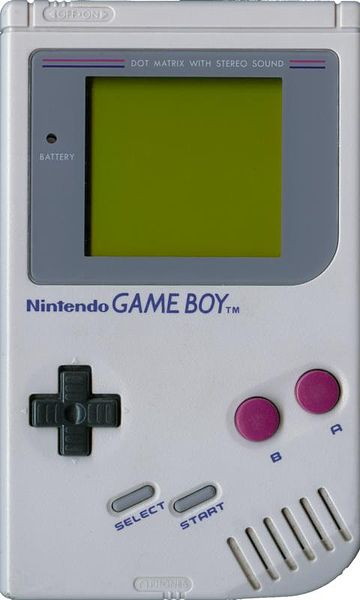
\includegraphics[height=5cm]{./Figuras/C1/c1_360px-Gameboy.jpg}}
	\subfloat[\textit{Nintendo DS}]{
		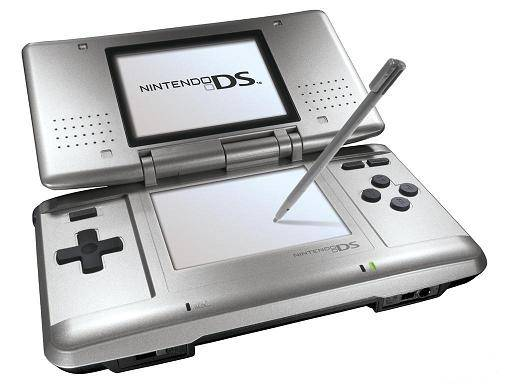
\includegraphics[height=5cm]{./Figuras/C1/c1_Nintendo_ds.jpg}}
	\caption{Videoconsolas de Nintendo: GBA y NDS}
	\label{fig_c1_nintendo1}
\end{figure}

\begin{figure}
	\centering
	\subfloat[\textit{Nintendo DS Lite}]{
		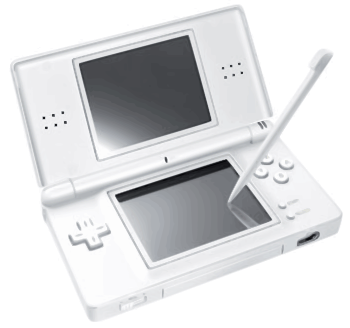
\includegraphics[height=5cm]{./Figuras/C1/c1_Nintendo-ds-lite.png}}
	\subfloat[\textit{Nintendo DSi}]{
		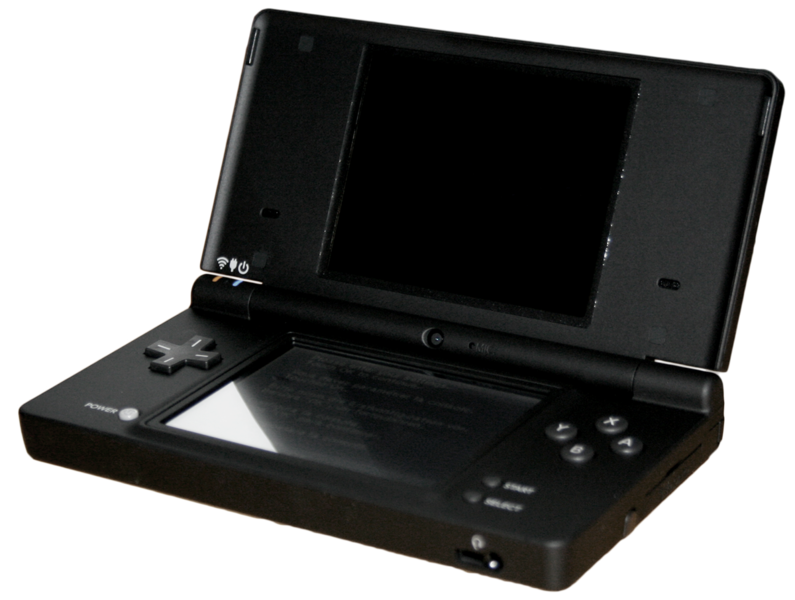
\includegraphics[height=5cm]{./Figuras/C1/c1_Nintendo_DSi.png}}
	\caption{Videoconsolas de Nintendo: NDSLite y NDSi}
	\label{fig_c1_nintendo2}
\end{figure}

\begin{figure}
	\centering
	\subfloat[\textit{Nintendo 3DS}]{
		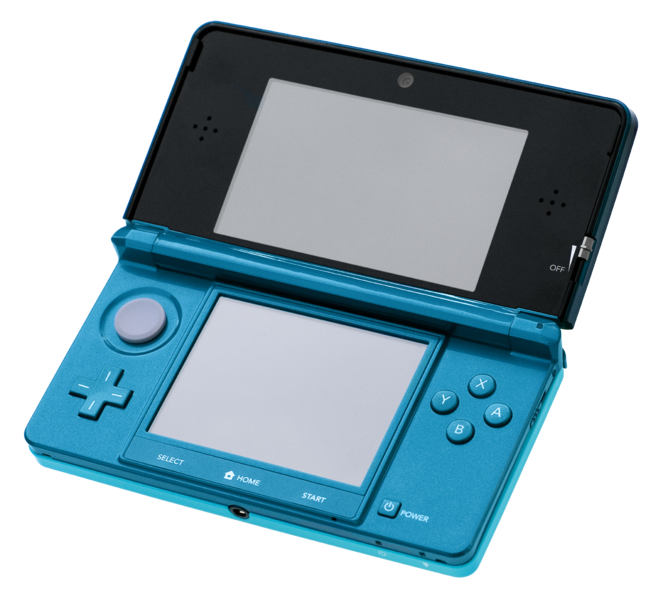
\includegraphics[height=4cm]{./Figuras/C1/c1_663px-Nintendo-3DS-AquaOpen.png}}
	\subfloat[\textit{Nintendo 2DS}]{
		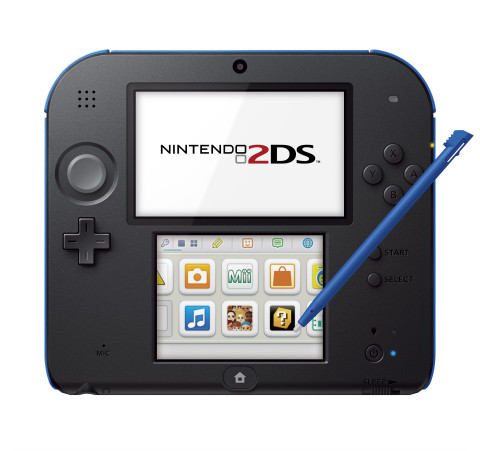
\includegraphics[height=4cm]{./Figuras/C1/c1_nintendo-2ds.jpg}}
	\subfloat[\textit{New Nintendo 3DS}]{
		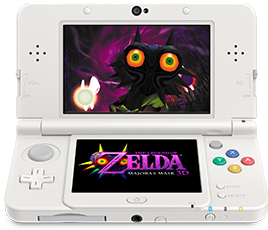
\includegraphics[height=4cm]{./Figuras/C1/c1_new-nintendo.png}}	
	\caption{Videoconsolas de Nintendo: N3DS, N2DS y NNew3DS}
	\label{fig_c1_nintendo3}
\end{figure}

% -----------------------------------------------------------------
% -----------------------------------------------------------------
% -----------------------------------------------------------------
% -----------------------------------------------------------------
\section{Hardware de la Nintendo DS (NDS)}

A continuación se describe el hardware de la \textit{Nintendo DS}:

\begin{itemize}
\item \textbf{Procesadores}: cuenta con dos procesadores, un ARM9 y un ARM7. El procesador ARM9 se encarga de la	lógica principal del programa, mientras que el ARM7, como procesador secundario, se encarga básicamente de gestionar el audio, la red inalámbrica (\textit{WiFi}) y algunas teclas. El hecho de que la consola NDS cuente con dos procesadores implica	la generación de dos ejecutables distintos, uno para cada procesador. El ejecutable del ARM7 actúa como esclavo del ARM9, atendiendo peticiones de reproducción de sonido o comunicaciones vía WiFi.
%	
\item \textbf{Memorias}:
	\begin{itemize}
	\item Memoria principal: tiene un tamaño de 4 MB. Dicha	memoria almacena el ejecutable para el ARM9, así como la gran mayoría de datos del ejecutable. Ambos procesadores pueden acceder a esta memoria en cualquier momento. Si ambos intentan acceder a la vez, será el que tenga mayor prioridad el que accede, quedando el otro a la espera.
	%
	\item Memoria de vídeo \textit{VRAM}: tiene  656 KB  distribuidos en  9 bancos de memoria de vídeo, que se pueden usar con diferentes propósitos. A lo largo de las sesiones de prácticas se verán más detalles de esta memoria de vídeo.
	%
	\item Otras memorias: tiene las pseudo-cachés \textit{WRAM} e \textit{IWRAM} de 96Kb, una memoria \textit{RAM} adicional para la \textit{BIOS} y una memoria virtual para vídeo (\textit{Virtual Video RAM}). 
	\end{itemize}
%
\item \textbf{Gráficos}: el hardware de vídeo se compone de dos núcleos gráficos 2D, uno	principal (\textit{main}) y otro secundario (\textit{sub}). Dichos núcleos se diferencian únicamente en que el motor principal puede \textit{renderizar} tanto la memoria de vídeo virtual sin utilizar el motor 2D, como mapas de bits de 256 colores, así como utilizar el motor 3D para el renderizado de alguno de sus fondos.
%
\item \textbf{Sonido}: dispone de altavoces estéreo y cuenta con 16 canales de audio independientes.
%
\item \textbf{Comunicación inalámbrica}: soporta el estándar de protocolo de comunicaciones \textit{IEEE 802.11}. El rango de comunicación inalámbrica varía de 10 a 30 metros, dependiendo de las circunstancias.
%
\item \textbf{Entrada/Salida}: tiene un puerto para cartuchos de juegos de Nintendo DS y otro para juegos de Game Boy Advance2. La NDS cuenta con una entrada para auriculares estéreo y otra entrada para micrófono.
%
\item \textbf{Doble pantalla}: las dos pantallas LCD son de 3 pulgadas. La pantalla inferior emplea tecnología táctil.
%
\item \textbf{Temporizador}: cuenta con un reloj de tiempo de real, que puede ser utilizado por una aplicación o juego para definir diferentes respuestas dependiendo de la hora del día.
\end{itemize}
